\chapter{Data Mining in Nearby Galaxies}
\label{ch: paper3}
%----------------------------------------------------------------------------------------
%----------------------------------------------------------------------------------------
%----------------------------------------------------------------------------------------
%Intro
%----------------------------------------------------------------------------------------
%----------------------------------------------------------------------------------------
%----------------------------------------------------------------------------------------
\section{Introduction} 
% Nearby galaxies and their importance 
Nearby galaxies play an important role in our understanding of galaxies' formation and evolution.
Nearby galaxies are defined as those close enough that we are able to observe their structure and composition in detail.
As a result, many studies have been devoted to finding relations between physical properties of galaxies, such as morphology, star formation rate (SFR), stellar mass, metallicity, and amount of gas, both for spatially-resolved regions and galaxies as a whole~\citep[e.g.][]{Wong13,Leroy08}, and many others use these results in analyzing observations of high-redshift galaxies~\citep[e.g.][]{Freundlich13,Walch11}.
Surveys such as KINGFISH~\citep{Kennicutt11} and THINGS~\citep{Walter08} have made observations of nearby galaxies in various wavelengths and from these data we can measure physical properties such as stellar mass, star formation rate (SFR), dust mass, and gas mass~\citep[e.g.][]{Eskew12,Dale09,Calzetti07}.

% A little bit about M31 and previous studies in M31.
The Andromeda galaxy (M31), at a distance of $\sim$~0.78~Mpc, is the closest spiral galaxy to the Milky Way~\citep{McConnachie05}.
Images of this galaxy provide us with a detailed view of the inside of a spiral galaxy as seen from an external perspective.
M31 has been observed by many telescopes including the {\textit {Hubble}}, \Spitzer and \Herschel space telescopes. %Els: Use the correct names for telescopes?
\cite{Barmby06} used data from the \Spitzer Infrared Array Camera \citep[IRAC;][]{Fazio04} to show the spatial distribution of Polycyclic Aromatic Hydrocarbons (PAHs) in the interstellar medium (ISM) of M31.
Using data from the Multiband Imaging Photometer for Spitzer (MIPS) instrument, \cite{Gordon06} studied the morphology of M31's dust.
\cite{Azimlu11} and \cite{Sanders12} catalogued and studied \hii~regions of M31.
\cite{Draine14, Mattsson14, Viaene14, Smith12} and~\cite{Fritz12} used \Herschel data to study dust in the ISM of the galaxy.
Properties of the current stars in the galaxy were studied by many groups~\citep[e.g.][and references therein]{Tamm12,Dalcanton12,Massey07}.
\cite{Rahmani16, Ford13} and \cite{Tabatabaei10} measured the spatially-resolved SFR in M31 in order to study star formation laws, and~\cite{Dim15} and \cite{Kapala15} used infrared spectroscopy to study PAHs and atomic and molecular line emission in the ISM.

Although all these studies measured some properties of M31, or answered specific scientific questions about this galaxy, we still do not have a complete picture of underlying processes in the galaxy.
What is the correlation between PAHs and SFR, dust mass, and gas mass in M31? 
Are PAH features in M31 similar or they can be divided into various groups? If so, what are the properties of each group?
Does the intensity of PAH emission depend on location or global galaxy properties? 
The properties of M31 that derived in various studies and observational data of this galaxy can be used for a knowledge discovery and data mining study.
The Pinwheel Galaxy (M101), with distance of 6.7~Mpc~\citep{Freedman01}, is another nearby galaxy that has been well-observed and studied~\citep[e.g. ][and references therein]{Kennicutt11,Dale09, Leroy08, Gordon08}.
M101 is a large spiral galaxy with several \hii~regions and a large metallicity gradient from centre to outskirts~\citep{Kennicutt03}.
Since the observational data from M31 and M101 are similar, M101 is a suitable addition to M31 data for a data mining study. 
Knowledge discovery and data mining methods are designed to extract hidden information from data and have been tested in many astronomical studies~\citep[e.g.][and references therein]{Ball10}.
However, this study is the first to use a data mining method on observations of nearby galaxies.

% data mining and clustering in general; when we have so many data and we want to map them
\cite{Ball10} gave an extensive review of data mining and machine learning algorithms and their usage in astronomy.
A data mining algorithm learns about data from training, which can be supervised or unsupervised.
Supervised training refers to methods that use examples of the desired output to learn about input data; these are valuable tools for classifying data with known target values.
Unsupervised methods train without any prior knowledge of output results: 
they work solely based on the underlying structure of the input data.   
The unsupervised methods are very useful tools in knowledge discovery studies, where we have limited pre-expectations for the data or when we want to make sure that we did not miss any valuable information in previous studies.

The purpose of the present work is to use M31 observations to provide new insights into nearby galaxies, with a focus on relations between PAHs and other properties of the galaxy,
as there are few studies on relations between properties of M31 with its PAH features.
\cite{Cesarsky98} studied PAH spectra observed by ISOCAM spectro-imaging in four regions in M31 and found that PAH features in M31 differ from those in other galaxies in having weak or no $6.2 - 8.6$~$\mu$m emission with enhanced 11.2~$\mu$m emission. 
However,~\cite{Dim15} using {\it Spitzer}/Infrared Spectrograph~\citep[IRS;][]{Houck04b} observations, found that the PAH spectra of M31 have the same features as the spectra of other nearby star-forming galaxies.
Those authors re-evaluated the ISOCAM data to compare them to IRS data and found that the earlier results were likely due to incorrect background subtraction.
Using IRAC imaging observations,~\cite{Barmby06} found good agreement between the M31 SFR derived using observed 8~$\mu$m luminosity with other 
star formation indicators such as \halpha and far infrared luminosity.
\cite{Draine14} found that the PAH abundance in M31 is almost constant up to a galactocentric radius of $\sim 20$~kpc.
With data mining techniques we address the question of whether,
compared to other galaxies, PAH features in M31 are unique as~\cite{Cesarsky98} claimed, or  are normal as ~\cite{Dim15} and \cite{Draine14} concluded.


%this project 1 M31 and its extensive data we do not have any SOM in nearby galaxies
In this project we apply the self-organizing map algorithm (SOM) to M31 data, training 1D and 2D networks.
Using networks with fewer neurons, we study the properties of the clusters and investigate relations between PAH features and other quantities in M31.
We create 2D SOMs from subsets of the data as well as all available data, which helps us to understand the effect on each input on the position of the clusters in the SOM.
We apply the 2D trained networks to the M101 data to study whether they have similar properties to M31 ones.
If our hypothesis is correct, we should be able to see that regions in M31 and M101 with the same positions in the SOM have the same properties.


We describe the SOM method in $\S$~\ref{sec: method_SOMN}. 
In $\S$~\ref{Sec: data_SOMN}, we present the observational data from M31 and M101 that we use in this study.
The results of the 1D SOM networks and the study of PAHs in M31 are presented in $\S$~\ref{Sec: 1d_cluster}.
In $\S$~\ref{sec: 2d_cluster}, we present the results of 2D SOM networks and their use in extracting information about other galaxies.
In $\S$~\ref{sec: summary}, we summarize our results and discuss potential future work in this subject.
%----------------------------------------------------------------------------------------
%----------------------------------------------------------------------------------------
%----------------------------------------------------------------------------------------
%Method
%----------------------------------------------------------------------------------------
%----------------------------------------------------------------------------------------
%----------------------------------------------------------------------------------------
\section{Method}
\label{sec: method_SOMN}
\subsection{Choosing an Algorithm}

Some of the most tested methods of data mining in astronomy are artificial neural networks (ANNs)~\citep[e.g.][and references therein]{Hossein14,Hossein16}.
ANNs are spiered to work in the same way that the neurons work in a human brain.
These are networks of interconnected neurons (nodes), in which all of the connections are weighted.
These networks are used to study nonlinear and complex relations between input and output data.
One of the most well-known unsupervised neural networks in astronomy is a Kohonen self-organizing map (also called self-organizing map, or SOM).
SOMs visualize complex data~\citep{Kohonen82} and show simple geometrical relationships in non-linear high dimensional data~\citep{Kohonen98}.
The result of a SOM is a 1D or 2D network of neurons, which shows the positions of clusters and their relative distance.
Since the 1990s, many studies have utilized SOMs for object classification and clustering (e.g. classifying quasars' spectra, star/galaxy classifications, gamma-ray burst clustering and light curve classification) and photometric redshift estimation~\citep[e.g.][]{Odewahn92, Hernandez94, Murtagh95, Maehoenen95,Scaringi09,Geach12,Fustes13,Meusinger16,Rahmani16b}.

The K-means algorithm, SOMs, and hierarchical clustering are the main unsupervised methods that are used in astronomical studies~\citep[e.g.][]{DAbrusco12, Aycha16}.
For K-means algorithms, the user must define the number of clusters and for and SOM algorithms the user defines the number of neurons, and the algorithms decide how to separate the data into clusters.
In the hierarchical clustering method, the user must define dissimilarity between the groups; the algorithm combines (or divides) existing groups based on their dissimilarity and creates a hierarchical structure. 
Comparing the SOMs, K-means and hierarchical clustering methods shows that in some cases the hierarchical clustering method mis-classifies the data~\citep[][and references therein]{Mangiameli96}.
We chose the SOM method over the K-means method due to the fact that SOMs not only cluster data, but also show similarities and dissimilarities between the clusters.
Therefore, we can cluster our sample data and study the underlying structure simultaneously.

     
    \subsubsection{Algorithm of SOM} 
   \label{sec: algorithm_somz}
    The self-organizing map is a clustering method which reduces the dimension of the data, usually to one or two dimensions (1D or 2D), while preserving topological features of the original dataset.
    The result of an SOM is a set of nodes (neurons) that are arranged in a 1D or 2D arrays \citep{Kohonen98}. 
    Each node may contain one or more samples from the input data.
    The distance between the nodes represents similarity or dissimilarity of the underlying samples, i.e., similar data are closer together in the array and the distance between two nodes is related to the dissimilarity of their samples.
    A weight vector ``\boldit{W}" with the same dimension as the input data is associated with each node and will be varied during the training process.
    This vector is the key factor in determining the position of the nodes in a map.
    \cite{Geach12} presented the application of the SOM and discussed its algorithm in detail.
    In this section we briefly discuss the algorithm of SOM, how we create our maps and a present a  test model which will help interpretation of our results. 
   
     Assume we have a dataset which contains vectors, \boldit{V} $\in \Re^n$, and we want to map them on an S1 by S2 map. 
     We start by creating S1 $\times$ S2 empty neurons. 
     The initial arrangement of these neurons depends on the map's topology provided by the user.
     In the case of 1D maps, since each neuron has two immediate neighbours, the topology of the map does not have any effect on the final result and any topology can be chosen.
     However, in 2D maps, the shape of the neurons specifies the number of immediate neighbours for each neuron and it is up to user to choose the most suitable shape based on the data.
     In this paper, we choose hexagonal topology, which gives each neuron six neighbours, and provides more interactions between neurons.
     Initially a random weight vector, \boldit{W} $\in \Re^n$, will be assigned to each node.
     The process of creating SOM happens over a series of $N$ iterations. 
     During each iteration the weight vectors might change according to the Kohonen learning rule (equation~\ref{equ: weight adj_SOMZ}). 
      In each iteration, the SOM code:
     \begin{enumerate}
        \item chooses a random vector from the dataset ($V_i$).
        \item calculates the Euclidean distance for each node, $j$, as  $D_j^2= \sum_{i=0}^{i=n} (V_i - W_i)^2$, and finds a neuron with minimum $D_j$, (``$D_{j_{min}}$"). This neuron is the winner node and is called the Best Matching Unit (BMU). 
        \item  computes the radius of the neighbourhood of the BMU to find nodes within this radius. The weight vectors of these nodes will be affected in the next steps. The radius of the neighbourhood is arbitrary and can be set to be as high as half of the SOM size. It then decays exponentially over each iteration as
        \begin{equation}
            r^t_{BMU} = r^0_{BMU}e^{(-t/\tau)}
        \end{equation}
        where $\tau$ is a decay constant and is usually set to be the same as the number of iterations, $N$. $r^0_{BMU}$ and $r^t_{BMU}$ are the radii of the neighbourhood at 0th and $t$th iteration, respectively. 
        \item changes the weight vectors of the BMU and all the nodes within $r^t_{BMU}$ as:
        \begin{equation}
            \label{equ: weight adj_SOMZ}
            w(t+1)=w(t)+L(t) \times R(t) \times(v(t)-w(t))
        \end{equation}
        where $L(t) = L_0 e^{(-t/\tau)}$ is the learning factor, which prevents the divergence of the SOM and $R(t)=\exp(-\frac{D_j^2}{2r^t_{BMU}})$ is the influence rate. $R(t)$ determines how the weight of each node in the neighbourhood of BMU will change.
     \end{enumerate}
     These steps are then repeated $N$ times.
     
\subsection{Creating Self-Organizing Maps}
\label{sec: create_som}
     In order to create SOMs, we use {\sc matlab} neural network toolbox~\citep[NNT,][]{matlabtolbox}.
     
     SOM in {\sc nnt} can be created by {\sc newsom} or {\sc selforgmap} library, both of which work in two phases, an ``ordering phase" and a ``tuning phase". 
     The first phase is called the ``ordering phase" and
     starts with maximum neighbourhood distance and an initial high learning factor (usually 0.9) is provided by the user. 
     The ordering phase continues for a requested number of iterations.
     During the iterations, the learning factor decreases to the tuning phase learning factor and the neighbourhood distance reaches that of the tuning phase as well.
     Both the learning factor and the neighbourhood of the tuning phase are set by the user. 
     The amount by which these two factors change in each iteration depends on the number of iterations.
     
     In the second, or ``tuning'' phase,
     the neighbourhood distance is kept at the user-defined minimum.
     The learning factor, however, decreases gradually.
     The gradual change in the leaning factor helps to fine-tune the topology results, leading to a more stable SOM. 
     To allow the fine tuning, the number of iterations in this phase must be much larger than the that of the ordering phase.
     We chose the number of epochs in the tuning phase to be 3 times the number of epochs in the ordering phase.
     
     To present our results, we use {\sc nnt}'s built-in plotting tool.
     Specifically, we use two of the plots in this tool: a hits map, which shows the number of times each neuron has became the winner (hits), and a distance map, which shows the distance between those neurons.
     In the maps, the purple hexagonal shapes represent the neurons. 
     The distances in a distance map are shown by the grey cycle colours:
     the darker the colour, the larger the distance between neurons.
     In the hit maps, neurons with zero hits are left empty.
      
    The sizes of the SOM maps are arbitrary and there are no rules regarding choosing one over the other. 
    \citet{Vesanto05} suggested that a total number of $5\sqrt{n}$ neurons is a sufficient size, but users usually choose the size of the grids based on their dataset and their application of the results.
\subsection{Mock Sample}
\label{sec: mock_sample}
 
         \begin{figure}
                \centering
                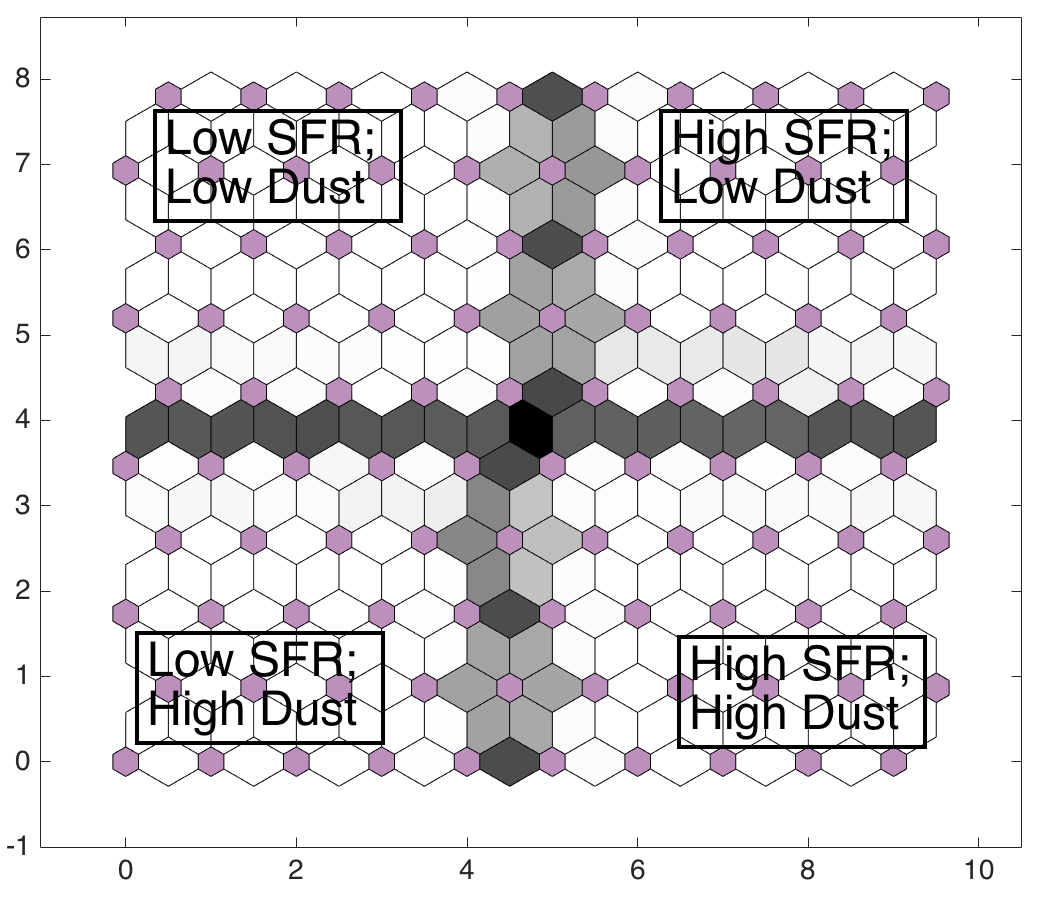
\includegraphics[width=\textwidth]{../image_paper3/images0.01/mock_sample.png}
            \caption[Self-organizing map of the mock sample]{SOM of the mock sample. The axes show the position of the neurons. Hexagonal shapes represent the neurons. The grey-scale colours show the differences between neuron weights, where white is the minimum difference and black is the maximum one.}
            \label{fig: sample}
        \end{figure}
 
To show how self-organizing maps work, we created a mock sample containing only a few regions.
Each sample had two properties: the amount of dust and the star formation rate, where the possible values were
either 0 or 1 for low or high SFR, and 0 or 0.5 for a low or high amount of dust. 
 We generated an SOM from the sample with a size of $10 \times 10$, using the method described in Section~\ref{sec: method_SOMN}.
 Fig.~\ref{fig: sample} shows the SOM of the mock sample. 
 The axes show the position of the neurons in a $10 \times 10$ network and the hexagonal shapes (depicted by purple hexagons) are the neurons.
 
Using this method, as expected, we are able to divide the mock sample into 4 distinct groups. Their boundaries are shown by grey colours in Fig.~\ref{fig: sample}: regions with high SFR and high dust content, regions with low SFR and high dust content, regions with high SFR and low dust content, and regions with low SFR and dust content. 
In Fig.~\refthere ha{fig: sample}, the upper part belongs to regions with low dust content, while the lower part belongs to regions with high dust content.
The left part of the plot is where regions with low SFR belong and the right side is for high SFR regions.
Grey to black colours show the border between regions.
This network is considered to be a trained network, and can be used to cluster any new data set with similar entries.

Having two regions with exactly the same values in all their quantities with real data is extremely unlikely. 
If, in an input data set, there are two entries with similar (but not identical) values in all dimensions, one can find a network that separates these two entries in two groups.  
However, in case of multiple similar entries in a dataset, the number of neurons must be much higher than the number of entries for complete separation.
Therefore, the user learns about similarity or dissimilarity of members of the input dataset based on the ratio of the number of entries in the dataset and  the number of neurons. 

%----------------------------------------------------------------------------------------
%----------------------------------------------------------------------------------------
%----------------------------------------------------------------------------------------
%DATA
%----------------------------------------------------------------------------------------
%----------------------------------------------------------------------------------------
%----------------------------------------------------------------------------------------
\section{Study Sample}
\label{Sec: data_SOMN}

Our study includes 10 regions in M31 (Fig.~\ref{fig: regions in m31}) and 8 regions in M101 (Fig.~\ref{fig: regions in m101}). 
These specific regions were chosen for the availability of \Spitzer/IRS 5--15$\mu$m  spectroscopy covering the PAH emission bands.
Besides PAH band strengths, for each galaxy, we use spectroscopic and photometric observations as well as their derived properties, such as SFR, stellar mass, dust luminosity (L$_{\rm dust}$), dust mass, metallicity, and gas mass.
Table~\ref{tab: data} shows the full list of data for both M31 and M101.
All data were divided by the area of their region (in arcsec$^2$), to remove the distance factor from the data and compare values across galaxies.
Since the spatial resolution of the observations varies from as small as $<1$\arcsec to as high as 60\arcsec $\times$ 90 \arcsec, any attempt to match resolution would have caused a loss of information in some of the input quantities (e.g. the spectroscopic data).
In this project we used flux per unit area, which the convolution methods conserve~\citep{Aniano12}, as the input data.
Therefore, we did not perform any resolution matching and used data at their original resolution.

    \import{../image_paper3/text_files/tables/}{tab_data.tex}

    \begin{figure}
  \begin{subfigure}[b]{\textwidth}
        \centering
        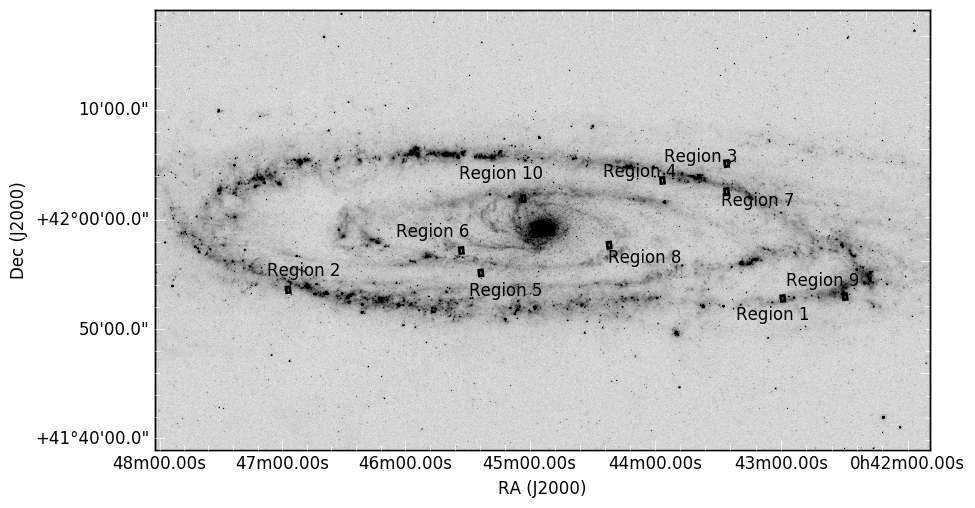
\includegraphics[width=0.97\textwidth]{../image_paper3/images0.01/M31/M31.png}
        \caption{MIPS~24 $\mu$m image of M31, with positions of 10 regions studied.}
        \label{fig: regions in m31}
    \end{subfigure}
    \hfill
    \begin{subfigure}[b]{\textwidth}
        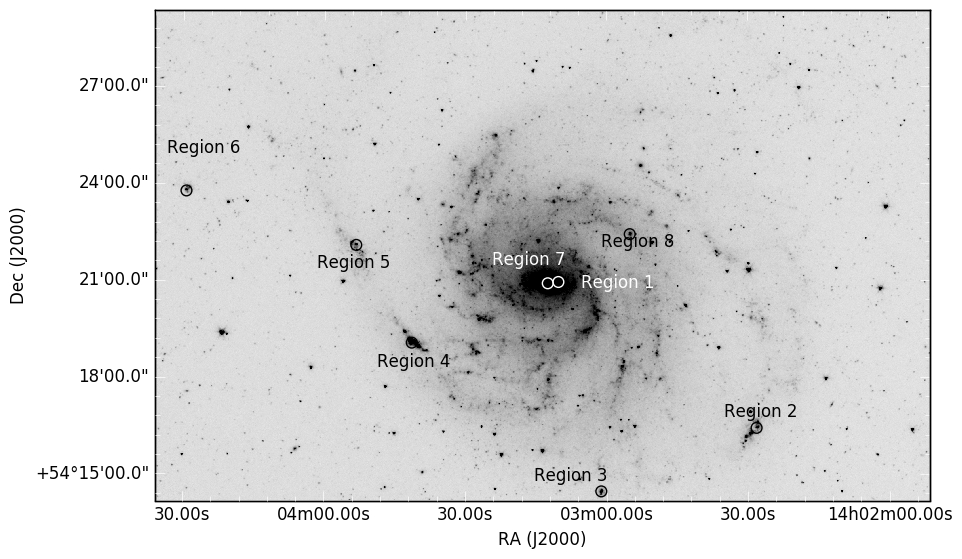
\includegraphics[width=\textwidth]{../image_paper3/images0.01/M101/M101.png}
        \caption{IRAC 3.6 $\mu$m image of M101, with positions of  8 regions studied.}
    \label{fig: regions in m101}
    \end{subfigure}
    \caption[Position of the data in M31 and M101]{Position of the data in M31 (a) and M101 (b).}
\end{figure}

    \subsection{M31 Observations}
     \label{Sec: data_M31_SOMN} 
     
     \cite{Dim15} used {\it Spitzer}/IRS observations to study PAHs in 10 regions chosen to span a range of mid-infrared flux ratios in M31 (Fig.~\ref{fig: regions in m31}). 
     Fluxes and equivalent widths of PAH and atomic line features were measured using the~\textsc{pahfit idl} tool~\citep{Smith07b}.
     \cite{Dim15} also measured metallicity and radiation hardness index (RHI) for these 10 regions.
     We used the measured PAH feature fluxes, metallicity and RHI of each region as the input for self-organizing maps.
     
    For the photometry part of the sample, we used the \GALEX \citep{Martin05} far-ultraviolet and near-ultraviolet (FUV and NUV) channel images; \halpha~(6574.7\AA), \sii~(6730.72\AA) and \oiii~(5024.9\AA) narrow band images~\citep{Massey07}, IRAC 3.6, 4.5, 5.8 and 8.0~$\mu$m images~\citep{Barmby06}; MIPS~24 and 70~$\mu$m~images~\citep{Gordon06}; and PACS 100 and 160~$\mu$m and SPIRE 250, 350, and 500~$\mu$m~\citep{Fritz12} images.
     The units of all fluxes were converted to W~m$^{-2}$ in order to be the same as the PAH fluxes.
     $^{12}$CO (J:$1\rightarrow0$) line emission images~\citep{Nieten06} and atomic gas (\hi) 21~cm emission images from~\cite{Chemin09} were added to the input data. 
     For derived values, we utilized SFR(FUV + 24$\mu$m) measured using combination of FUV and 24$\mu$m emission, stellar mass, molecular gas mass, atomic gas mass, total gas mass, and total infrared (TIR) luminosity (L$_\mathrm{TIR}$) from~\cite{Rahmani16}, and L$_\mathrm{dust}$ and dust mass from~\cite{Draine14}.
     
    \subsection{M101 Observations}
    \label{Sec: data_M101_SOMN} 
    
     \cite{Gordon08} measured PAH fluxes and RHI for M101 in 8 star forming \hii~regions (Fig.~\ref{fig: regions in m101}).
     Metallicities of 6 of the 8 regions were measured by~\cite{Kennicutt03} and the other two by~\cite{Gordon08}.
     We used the NED~\footnote{The NASA/IPAC Extragalactic Database (NED) is operated by the Jet Propulsion Laboratory, California Institute of Technology, under contract with the National Aeronautics and Space Administration.} website to gather imaging observations of M101, including 
      \GALEX FUV and NUV~\citep{depaz07}, IRAC 3.6 -- 8.0~$\mu$m, MIPS~24 and 70~$\mu$m~\citep{Dale09}, and PACS~100 and 160~$\mu$m and SPIRE~250, 350, and 500~$\mu$m emission from~\cite{Kennicutt11}.
     As with M31, we used $^{12}$CO (J:$1\rightarrow0$) line emission images~\citep{Helfer03} and atomic gas (\hi) 21~cm emission images from \cite{Walter08}.
     We calculated SFR(FUV + 24$\mu$m), stellar and total gas mass maps using the same methods as for M31.
     
     \subsection{Preparing Data for Data Mining}
    
     Correlations between some of single-wavelength emission and galaxy properties are well-known.
     Emission in the 3.6$\mu$m band traces the old stellar population very well~\citep[e.g.][]{Smith07a,Leitherer99} and it can be used to calculate the stellar mass~\citep{Eskew12}.
     FUV, \halpha, and TIR emission are indicators of star forming regions.
     In this project, we used the SFR traced by the FUV emission, corrected for foreground stars using NUV emission and for dust extinction using 24~$\mu$m emission.
     Total infrared emission is calculated from a modified version of~\cite{Draine07} calibrations using using 8, 24, 70, and 160~$\mu$m emission~\citep{Boquien10}.
    
    
    We removed all the observed data that were used to calculate galaxy properties from the input sample, to guarantee that they have not been used in multiple forms.
    To have prior knowledge of the M31 data set, 
    we computed the Pearson correlation coefficients between input measurements.
    Fig.~\ref{fig: cor_all} shows the Pearson correlation coefficients with a confidence level of 95 per cent. 
    If the significant level of correlation becomes smaller than 0.05 (5 per cent), the correlation is marked as insignificant. 
    All the PAHs correlate with one another very well.
    They are also highly correlated with the SPIRE and PACS emission, L$_\mathrm{dust}$, L$_\mathrm{TIR}$, SFR and metallicity.
    The fluxes from PAHs 7.7, 8.3, 12.7 and 17~$\mu$m show a weak anti-correlation with RHI.
    In general, PAHs in our data set are highly correlated with most of the other quantities. 
    
      \begin{figure}
        \centering
        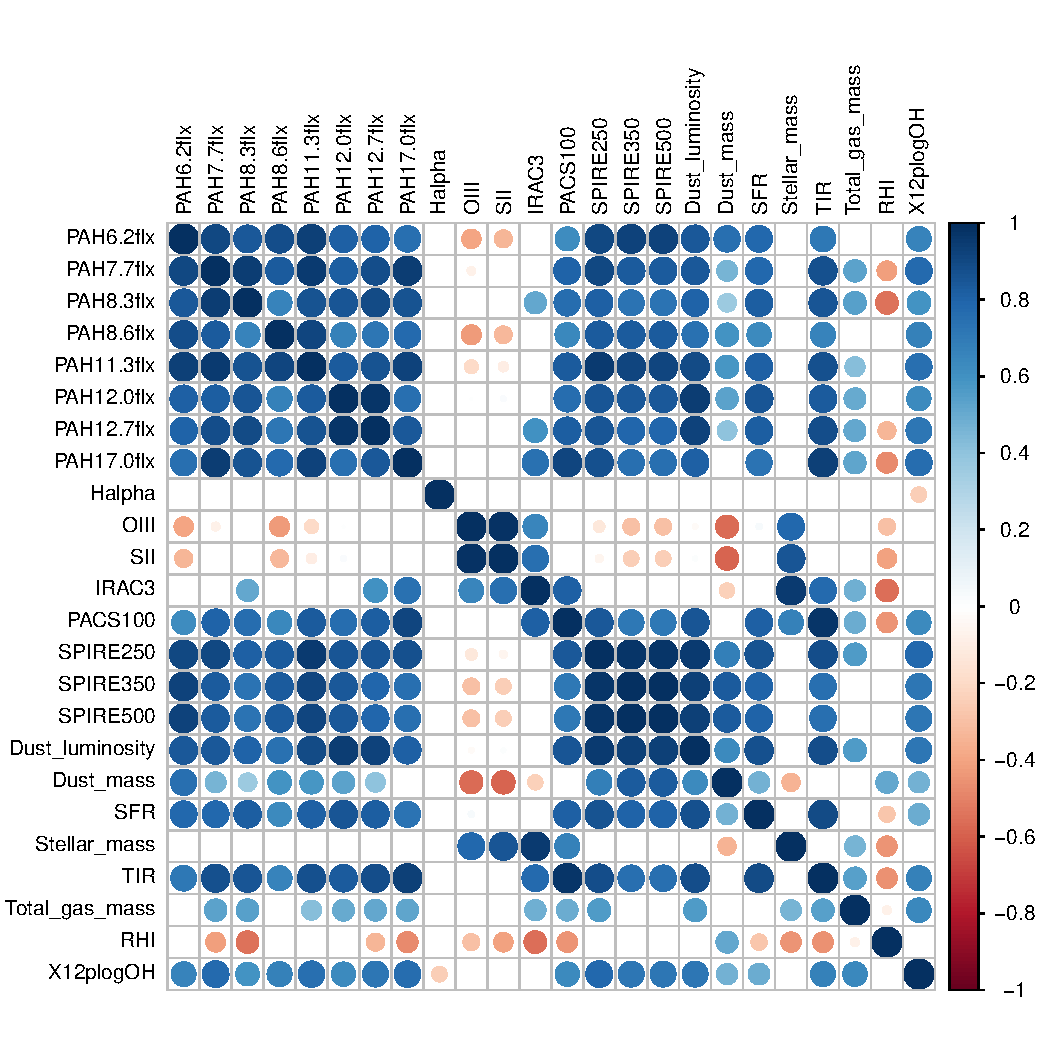
\includegraphics[width=\textwidth]{../image_paper3/images0.01/cor_plots/M31_all_derived_ones_core_plot_for_paper.pdf}
        \caption[Pearson correlation coefficients for data from 10 regions in M31]{Pearson correlation coefficients with a confidence level of 95 per cent for all data from M31. The colours and circle sizes show the Pearson correlation coefficients where large blue circles are 1, which means highly correlated, and large red circles are $-1$, which means highly anti-correlated quantities. The boxes with non-significant correlations were left empty.}
        \label{fig: cor_all}
    \end{figure}
 
 %----------------------------------------------------------------------------------------
%----------------------------------------------------------------------------------------
%----------------------------------------------------------------------------------------
%Result Part 1: 1D SOMs
%----------------------------------------------------------------------------------------
%----------------------------------------------------------------------------------------
%----------------------------------------------------------------------------------------
\section{One-Dimensional Self-Organizing Maps}
    \label{Sec: 1d_cluster}
%Why 1D maps are useful
    The purpose of  exploring the M31 data with 1D maps is to monitor the general behaviour of the data. 
    One-dimensional SOMs can have the minimum number of clusters, $1\times2$, up to the highest number of clusters possible (infinity). %Els asked what is maximum possible #
    In a small sample like ours, smaller grid SOMs are very useful to find correlations that cannot be found without  clustering the data.
    On the other hand, larger grid 1D SOMs are a helpful tool to get quick insight into the data.

    \subsection{Clustering M31 Data}

        In order to monitor how the data behave, we created SOMs with two to fourteen neurons (Fig.~\ref{fig: M31_nets_1d}).
        The $1\times2$ network (Fig.~\ref{fig: M31_net_1by2}) shows how the M31 data can be divided into two broad categories.
        The $1\times14$ network (Fig.~\ref{fig: M31_net_1by14}) is the first network in which all the regions in M31 are completely separated.
        In the higher network sizes, regions have more space to be separated based on their differences. In going from the $1\times2$ to the $1\times14$ network the distance between M31 regions increases, until they are completely separated. 
        
        Fig.~\ref{fig: M31_net_1by2} shows that by forcing the regions in the M31 to be divided into two groups, regions 1, 2, 9 and 10 (shown in Fig.~\ref{fig: regions in m31}) occupy one neuron and the other regions occupy the other one.
        The medium grey colour between two neurons indicates that there are some similarities between two groups, but they are not very similar. 
        By increasing the size of the neurons to three, in Fig.~\ref{fig: M31_net_1by3}, we can see that region 2 separates itself from the other regions and occupies the middle neuron.
        The white colour between the two left neurons suggests that the regions which occupy these neurons are very similar to each other, while the black colour between the two right neurons indicates otherwise.
        
        %%%Talking about four right regions
        \cite{Dim15} showed that regions 1, 2, 9, and 10 have higher PAH fluxes compared to the other regions (fig.~5 in \citealt{Dim15}). 
        These regions also have relatively high intensities in all the mid-infrared and far-infrared bands and have high dust luminosity and dust mass.
        The higher values for these quantities could be the reason that these four regions become separated from the others in the $1\times2$ network.
        Regions 1 and 9 are in the 10~kpc ring, region 2 is slightly out of the 10~kpc ring and region 10 is in the bulge of M31; however, regions 3 to 8 are located out of the inner ring or the 10~kpc ring (Fig.~\ref{fig: regions in m31}).   
        The differences in their positions account for their difference in input parameters.
        Since region 10 is located in the bulge of M31 and has high surface brightness for most of the input values, regions 1, 2, and 9 to gradually move towards other regions and away from region 10 in the higher grid SOMs.
       
    \begin{figure}
    \begin{subfigure}[b]{\textwidth}
        \centering
        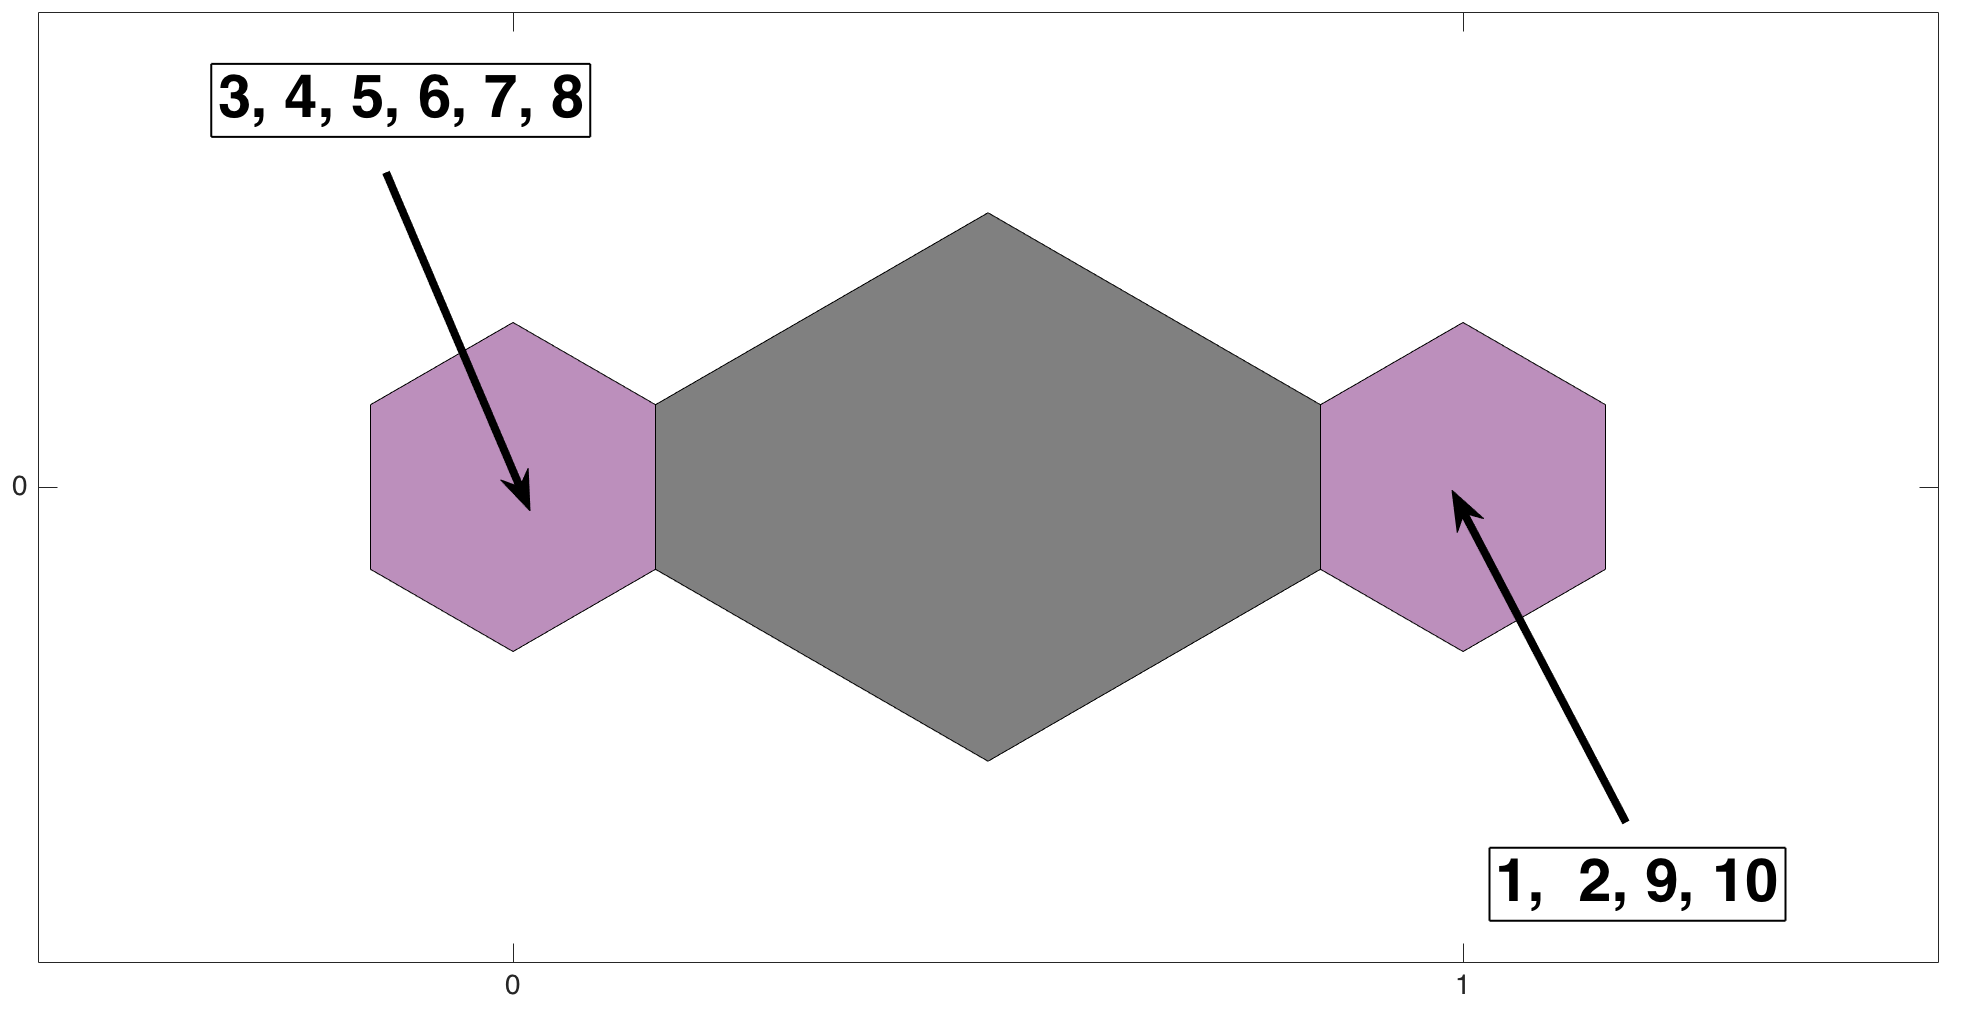
\includegraphics[width=\textwidth]{../image_paper3/images0.01/M31/1D/combine_1D_1by2_all.png}
        \caption{$1\times2$~network}
    \label{fig: M31_net_1by2}
    \end{subfigure}
    \hfill
    \begin{subfigure}[b]{\textwidth}
        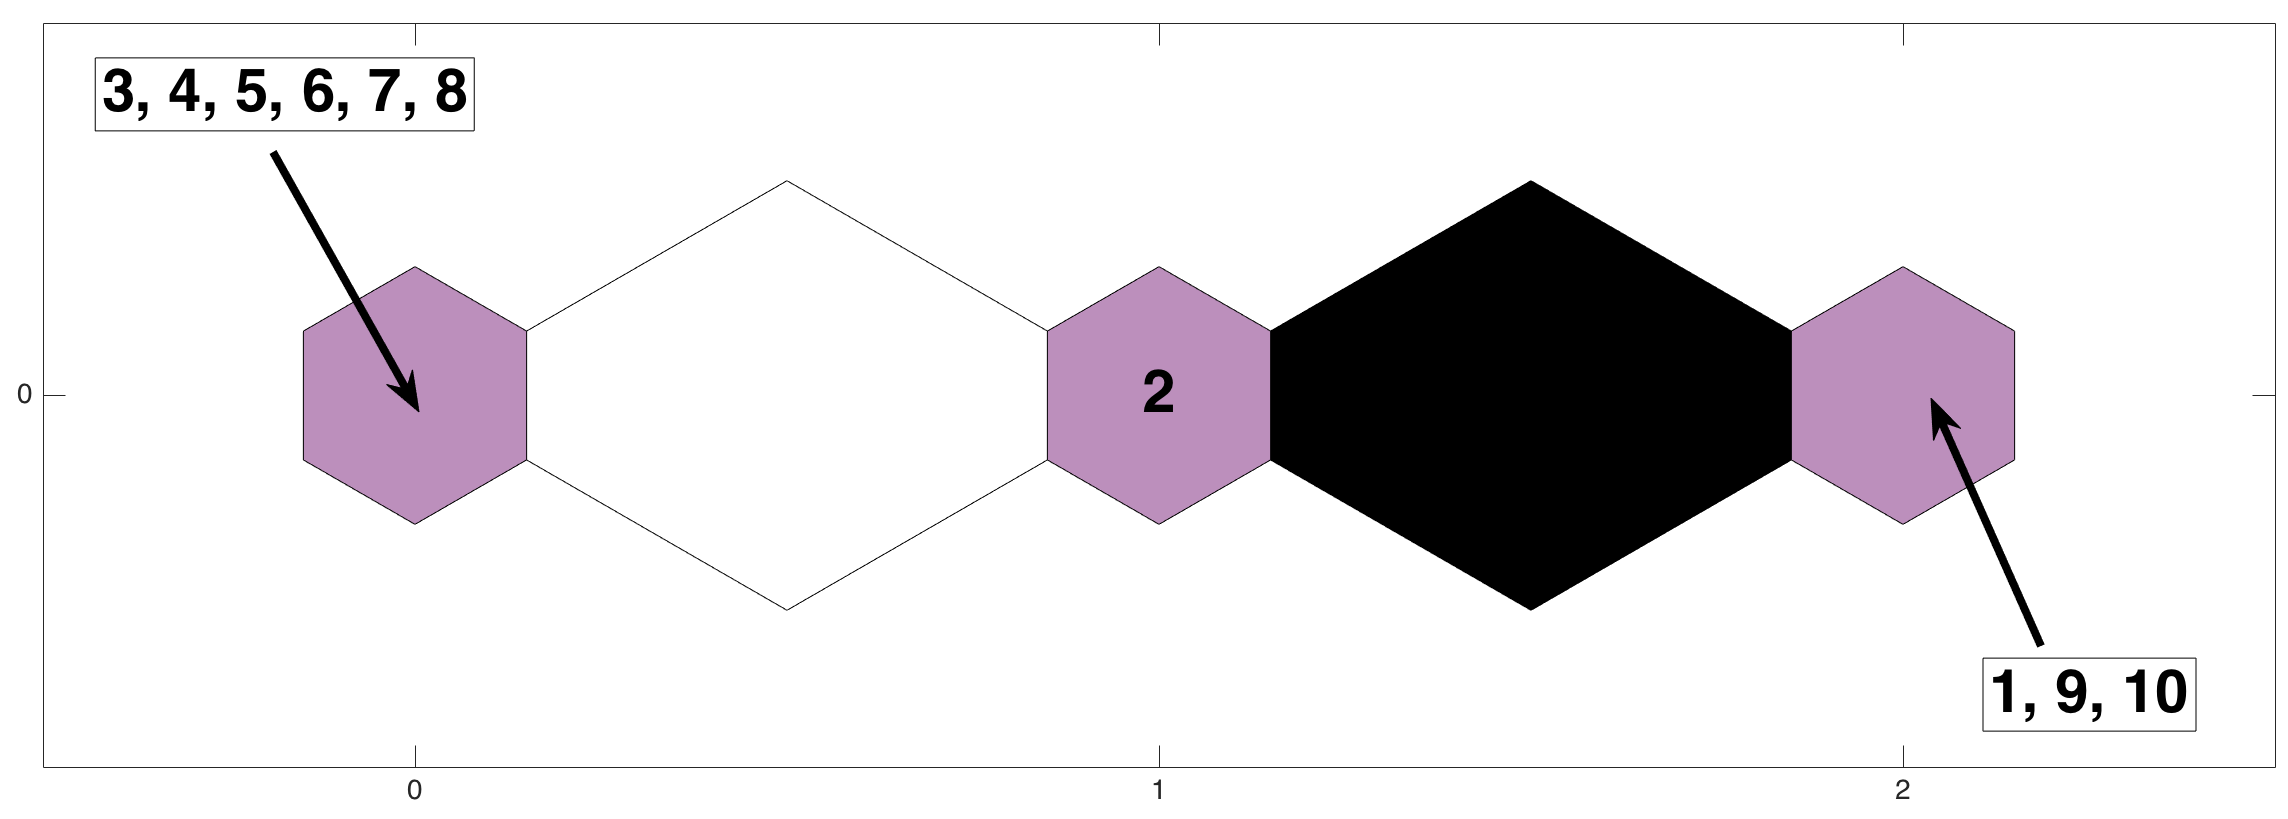
\includegraphics[width=\textwidth]{../image_paper3/images0.01/M31/1D/combine_1D_1by3_all.png}
         \caption{$1\times3$~network}
        \label{fig: M31_net_1by3}
    \end{subfigure}
    \hfill
    \begin{subfigure}[b]{\textwidth}
        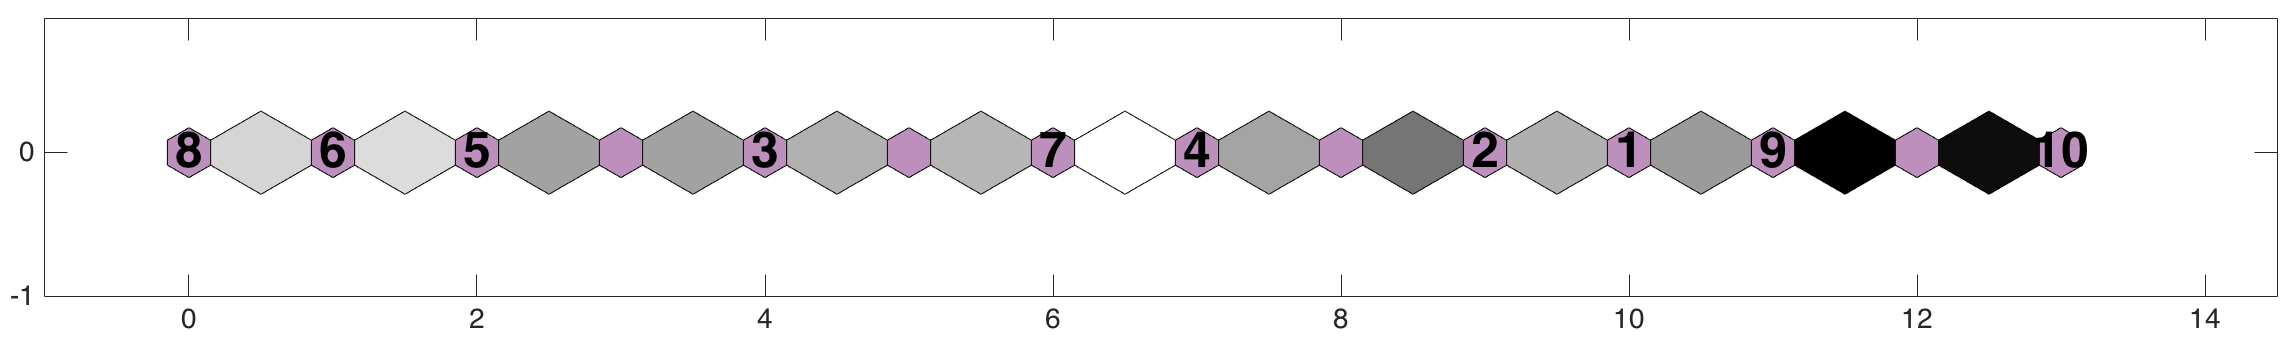
\includegraphics[width=\textwidth]{../image_paper3/images0.01/M31/1D/combine_1D_1by14_all.png}
        \caption{$1\times14$~network}
        \label{fig: M31_net_1by14}
    \end{subfigure}
   \caption[One-dimensional self-organizing map of M31 data]{SOM of the M31 data from $1\times2$, $1\times3$~and $1\times14$~grids. The axes show the position of the neurons. The purple hexagonal shapes represent the neurons. The grey scale colours show the differences between weight of the neurons, with white as the minimum difference and black as the maximum. The numbers in the plot show the M31 regions located in each neuron.}
   \label{fig: M31_nets_1d}
    \end{figure}
    

        %%Network 1by14
        The network with 14 neurons, in Fig.~\ref{fig: M31_net_1by14}, is the first network that has no neuron occupied by more than one M31 region.
        In a larger-grid SOM, the network pays more attention to smaller details and differences in the input data.
        Therefore, since at least 14 neurons are needed to separate all 10 regions in M31, we can conclude that some of the regions have very small differences.
        Regions that are located in similar areas (e.g. spiral arms, bulge, and 10 kpc ring) in M31, like regions 7 and 4 (see Fig.~\ref{fig: regions in m31}), are most likely to have more similarities with each other.
        In Fig.~\ref{fig: M31_net_1by14}, the right-most neuron is occupied by region 10.
        Two black colours between this region and the others indicate the large differences between this neuron and the other ones.
        Region 10 is located in the bulge of M31, and is physically separated from the other regions, which are mostly located around the inner or outer rings.
        The SOM shows that this region has completely different input values from the others: most of the values for region 10 are much higher than for the other regions, which is the main reason for its isolation.
        Region 8 occupies the right-most neuron in this network, suggesting that this region has the most differences from region 10.
        
    \subsection{Inside the Two Neuron Network}
        \label{sec: inside_the_2_neurons}
        Using self-organizing maps, we can identify hidden subgroups in our samples. 
        Each of these subgroups separates for a reason.
        This reason can vary from having higher values in some specific properties, as discussed in Section~\ref{Sec: 1d_cluster}, to some unknown correlations between data that cannot be seen in other groups or in the galaxy as a whole.
        To investigate the latter, we show in Fig.~\ref{fig: cor_cluster1} the Pearson correlation coefficients for the inputs from regions 3 to 8, which were clustered together in the $1\times2$ and $1\times3$ networks (see Figs.~\ref{fig: M31_net_1by2} and ~\ref{fig: M31_net_1by3}).
        
        \begin{figure}
        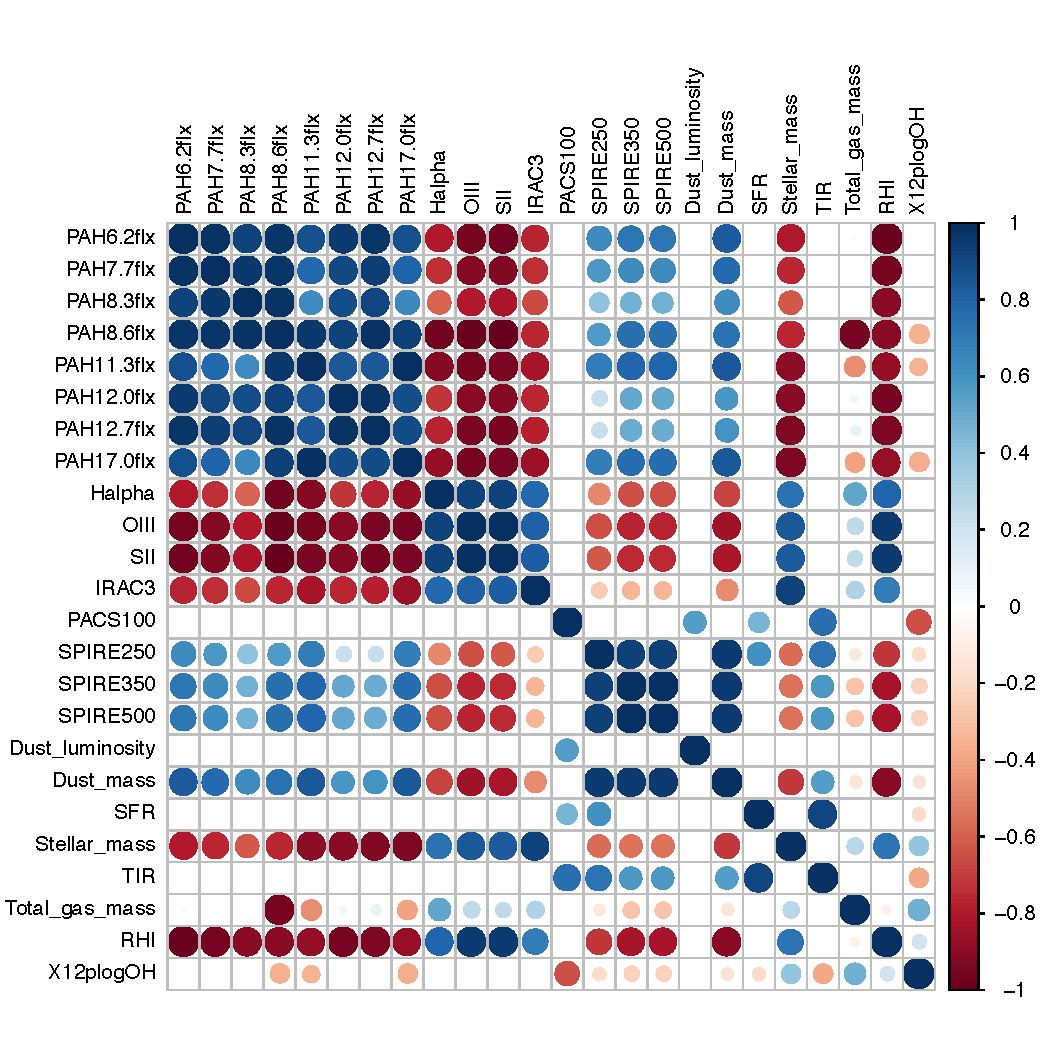
\includegraphics[width=\textwidth]{../image_paper3/images0.01/cor_plots/M31_derived_3_to_8_core_plot_for_paper.pdf}
        \caption[Pearson correlation coefficients for data from the clustered regions in M31]{Same as Fig.~\ref{fig: cor_all}, but here we used data from regions grouped in the left sides of Figs.~\ref{fig: M31_net_1by2} and ~\ref{fig: M31_net_1by3}. }
          \label{fig: cor_cluster1}
        \end{figure}
        
       
        Comparing the correlation coefficient plots for all 10 regions in M31 (Fig.~\ref{fig: cor_all}) and for the clustered data (Fig.~\ref{fig: cor_cluster1}) shows the differences between all 10 regions and clustered data and why regions 3 to 8 become separated from the other regions.
        The main features that differentiate these two plots are the anti-correlations between PAH features and RHI, stellar mass, \halpha, \sii, \oiii, and IRAC~5.8~$\mu$m~emission.
        Additionally, for the PAH fluxes in Fig.~\ref{fig: cor_cluster1}, there are no significant correlations with PACS~100~$\mu$m, L$_\mathrm{dust}$, L$_\mathrm{TIR}$, SFR, or metallicity.
        The PAH fluxes correlate with the SPIRE emission, but to a lesser extent than for the data from all regions.
        
        \cite{Calzetti10} mentioned that with increasing RHI in regions, metallicity and PAH equivalent widths decrease. 
        \cite{Dim15} investigated the correlation between PAHs features and both metallicity and RHI using the equivalent width of the 8~$\mu$m (combination of 7.7, 8.3, and 8.6~$\mu$m components) and the 7.7 and 11.2~$\mu$m features.
        They did not see any relations between PAHs and metallicity or RHI for 10 regions in M31.
        In Fig.~\ref{fig: cor_all}, we show that all the PAH fluxes correlate with metallicity, and PAH fluxes in the 7.7, 8.3 and 17.0~$\mu$m bands weakly anti-correlate with RHI.
        However, in Fig.~\ref{fig: cor_cluster1}, there is no correlation between the PAH fluxes and metallicity, but all of them strongly anti-correlate with RHI.
        \cite{Dim15} argued that the absence of (anti)-correlation between the PAH features and metallicity and RHI was related to a lack of data in low-metallicity regions.
        Although data from more regions would improve the results, our analysis shows that clustering data would show the missing (anti)-correlations.
        For example, for both clusters in Fig.~\ref{fig: M31_net_1by2},
        we can see anti-correlations between PAHs and RHI, but each of them has a different slope which removes the anti-correlation over all 10 regions. 
        
        Correlations between PAH features and SFR, and L$_\mathrm{TIR}$ are well-studied~\citep[e.g.][]{Peeters04,Tielens08}. 
        Many groups have used PAH features as a tracer of SFR by finding correlations between 
        PAH emission and SFR derived from extinction-corrected \halpha~\citep[e.g.][]{Calzetti07,Khramtsova13,Shipley16}.
        These correlations are seen in Fig.~\ref{fig: cor_all}, when we considered the data from all regions, but not in Fig.~\ref{fig: cor_cluster1} when considering the clustered data.
        Note that, since there are only 6 regions in the clustered data, even one outlier in the data may cause the correlation coefficient to become insignificant.
        Further analyses show that the absence of correlations between PAH fluxes and SFR is because of one outlier: region 6. Region 6 is located in a FUV-bright region, which breaks the correlations. 
        When we disregard this region, high correlations between 6.2 to 17.0~$\mu$m~PAHs and SFR (and L$_\mathrm{TIR}$) reappear.
        
     
        Strong anti-correlations between 6.2 to 17.0~$\mu$m~main PAH features and RHI, stellar mass, \halpha, \sii, \oiii, and IRAC~5.6~$\mu$m~emission in Fig.~\ref{fig: cor_cluster1} were not seen in Fig.~\ref{fig: cor_all} (even if we ignore the outlier values).
        Anti-correlations between PAH features and the \halpha, \sii, and \oiii~emission could be the result of one of the following. 
        First, the optical data are not corrected for dust extinction.
        The PAH features correlate with the amount of dust while \halpha~emission anti-correlates with the amount of dust due to extinction as suggested by \cite{Calzetti94}.
        Therefore, higher PAH fluxes imply higher dust abundance and less \halpha~emission, and the same holds for \sii~and \oiii~emission.
        Second is the possible effect of the structure of the observed regions.
        If the observed regions are located near the edge of \hii~regions we would expect to see more PAH and less \halpha~emission. 
        The anti-correlations between 6.2 to 17.0~$\mu$m~PAH features and RHI have been seen in other studies, as well~\citep[e.g.][]{Wu06, Gordon08,Calzetti10,Dim15}. 
        \cite{Wu06} suggested these anti-correlations could be the result of PAH destruction due to a high amount of harder radiation (thus higher RHI).
        On the other hand,~\cite{Gordon08} argued that the harder radiation could make the photodissociation regions (PDRs) smaller.
        The PAH features are mostly coming from the PDRs that are surrounded by \hii~regions, and the PAH features' underlying continuum emission is from the \hii~regions.
        Therefore, the lower flux of the PAH features could be the result of the smaller size of PDRs.%Els: If you have an harder radiation field, you destroy your smaller PAHs. Hence, simply a harder RHI does not argue for a smaller PDRs being more plausible. 
        The latter reason, which could also describe the anti-correlation between PAH features and \halpha~emission, seems to be the more probable one. 
        
        The strong anti-correlation between PAHs and stellar mass suggests that, a higher stellar mass decreases PAH emission. 
        In observations of M33,~\cite{Calapa14} showed that the 8/250~$\mu$m luminosity ratio correlates with 3.6~$\mu$m emission, which translates to stellar mass, %Els: I'm unfamiliar with the details of this translation. But if you look at individual HII regions or starforming complexes, I would think that the 3.6um flux is not dominated by the stellar light as the stars are too hot to have a large fraction of emission at these wavelengths?
        and conclude that the PAH emission traces the old stellar population.
        In Fig.~\ref{fig: cor_cluster1}, we see a weak anti-correlation between SPIRE 250~$\mu$m emission and the stellar mass.
        We see no correlation between 8/250~$\mu$m luminosity and stellar mass, either in the clustered data or in all 10 regions.

        To test that whether the anti-correlation between stellar mass and PAH emission is the result of the destruction of PAHs in high stellar mass regions, or that high stellar mass obscures PAH emission, we compared PAH abundance with stellar mass for the clustered regions.
        The ratio of 8/24~$\mu$m emission, which can be considered as a proxy for PAH abundances~\citep[e.g.][]{Sandstrom10,Khramtsova13}, does not anti-correlate with stellar mass for either the clustered data or all 10 regions.
        Therefore, we conclude that in our sample, stellar mass does not cause the destruction of PAHs.
        
        The anti-correlation between stellar mass and PAHs could be result of the position of the regions within M31.
        Regions 5, 6, and 8 are located in the stellar disk of the galaxy and have relatively high stellar mass and faint PAH emission. 
        According to~\cite{Dim15}, regions 5 and 8 are the only two regions in thesample that do not include an \hii~region, which could be the reason for the faint PAH emission for these regions.
        Regions 4 and 7 have similar quantities for both stellar mass and PAHs and region 3 has high PAHs and low stellar mass.
        Without data from more regions in M31, we cannot confidently say that higher stellar mass decreases PAH fluxes.
        
        
       Regardless of the fact that some of the (anti)-correlations in Fig.~\ref{fig: cor_cluster1} might have physical meaning, we have to mention that we only used 6 regions to calculate these correlation coefficients.
       The number of data points is not high enough to yield a strong conclusion about PAH properties in M31.
       However, we can conclude that since the correlation coefficients derived from the clustered data (Fig.~\ref{fig: cor_cluster1}) differ from the correlation coefficients derived from the data from all 10 regions (Fig.~\ref{fig: cor_all}), the SOM separated a hidden cluster of the data which has different properties.
        
        
        
 %----------------------------------------------------------------------------------------
%----------------------------------------------------------------------------------------
%----------------------------------------------------------------------------------------
%Result Part 2: 2D SOMs
%----------------------------------------------------------------------------------------
%----------------------------------------------------------------------------------------
%----------------------------------------------------------------------------------------
\section{Two-Dimensional Self-Organizing Maps}
 \label{sec: 2d_cluster}
    Although 1D networks are helpful to give a general idea about the data, neurons in 1D maps have a maximum of two neighbours, which can limit the usefulness of the results.
    In 2D networks, each neuron has two to six neighbours, which allows them to capture a complete picture of the complicated relations in the input data.
    Accordingly, we created $10\times10$ 2D networks to study the data in detail.
    As mentioned in previous sections, the sizes of SOMs are arbitrary and must be decided by users based on their goals for use of the SOM.
    
    In this section we chose $10\times10$ size despite knowing, from the size of our input data, that most of the neurons would be empty.
    Using 2D networks, we are mostly interested in the ability of the SOMs to show the underlying structure of the data rather than its clustering features.
    Fig.~\ref{fig: all_derived_ones} shows the 2D SOM of the M31 data.
    Similar to Fig.~\ref{fig: M31_net_1by14}, all the 10 regions are completely separated from each other in Fig.~\ref{fig: all_derived_ones}.
    \import{../image_paper3/text_files/image_texts/}{all.tex}
    
    Regions 4 and 7 are in the top left of Fig.~\ref{fig: all_derived_ones} with a very bright colour between their neurons, indicating that these two regions are very similar.
    Considering the position of these two regions in M31 (both right on the edge of the star forming rings in the galaxy), similarity of these two regions was predictable.
    The position of region 3 on the SOM is close to the position of regions 4 and 7, but with a darker colour between the nodes. 
    In Fig.~\ref{fig: regions in m31} it is clear that this region in M31 is physically closer to regions 4 and 7 than to any other region, but it is on the outer side of the star forming ring.
    Regions 5 and 6 are in the second neighbourhood (there are two neurons between them) of the SOM, with a medium gray colour between them.
    These two regions are physically located around the inner ring of the galaxy.
    Regions 8 and 6 are both in the inner ring of M31, but region 6's location has more star formation, which could be the main reason for their relative distance in the SOM in Fig.~\ref{fig: all_derived_ones}. 
    
    Regions 1 and 9 are close to each other and in the same side of the star forming ring. 
    However, region 1 is in an area of the galaxy with less diffuse \halpha~emission than region 9, which might be the reason for their distances in the SOM.
    Region 2 is more distant from other regions in the galaxy and located in the star forming ring.
    However, similar to regions 1 and 4, region 2 is located in an area of the galaxy with less diffuse \halpha~emission.
    Therefore, the place of region 2 in the SOM tends towards regions 1 and 4. 
    Region 10 is in the bulge of the galaxy, and its position on the SOM is isolated from all the other regions by a strip of a dark colours. 
    
    In order to analyse effects of any input data on the final SOM, in the following we created SOMs from various subsets of data.
    We compare results of the subsets with one another and with the SOM created from all data in Fig.~\ref{fig: all_derived_ones}.

    \subsection{Subsets}
    \label{sec: subsets}
    
            For analysing subsets, we create SOMs by using only PAH data, as well as using all data except the PAHs (Fig.~\ref{fig: PAHS_or_not_PAHs}).
             \import{../image_paper3/text_files/image_texts/}{PAHS_or_not_PAHs.tex}
            Comparing the SOM from all data in Fig.~\ref{fig: all_derived_ones} with the SOMs in Fig.~\ref{fig: PAHS_or_not_PAHs} shows that the general position of regions in those networks are the same. 
            Region 10 is in one corner of all three networks.
            However, in Fig.~\ref{fig: all_derived_ones} and Fig.~\ref{fig: wt_pahs}, region 10 is isolated from the other regions, while in Fig.~\ref{fig: only_pahs}, region 10 is much less isolated and only shows complete dissimilarity with region 8.
            Regions 9 and 10 are totally isolated in the SOMs in Fig.~\ref{fig: wt_pahs}, but in Fig.~\ref{fig: only_pahs}, they are more similar to other regions.
            In both SOMs in Fig.~\ref{fig: PAHS_or_not_PAHs}, there are dissimilarities between regions in M31 but in Fig.~\ref{fig: wt_pahs}, the colours are much darker than the ones in Fig.~\ref{fig: only_pahs}.
            This indicates that there is more similarity between the PAH features over all 10 regions than between the other input data.
            
            We increased the dimension of input data in Fig.~\ref{fig: only_pahs} (PAH-only data) gradually, by adding other quantities to the input data. 
            The order in which data were added is the same as the order in Fig.~\ref{fig: cor_all}, i.e. the SOM in Fig~\ref{fig: col3and11_dist} was created from PAH and \halpha\ emission as input data, the SOM in Fig~\ref{fig: col3and12_dist} created from PAHs, \halpha~emission and \sii~ continuum, and so on. 
            \import{../image_paper3/text_files/image_texts/}{col3byall.tex}
            
            At the beginning of each run, the SOM algorithm assigns a random weight to neurons that causes the overall position of regions in networks (even with the same input data) changes in each run of the algorithm.
            However, the position of each region relative to other regions changes dramatically only when the new sets of input data are given to the algorithm (assuming all the initial values for the run are unchanged).
            In all SOMs in Fig.~\ref{fig: inc_D_col3s}, region 10 is located in the corner of the SOMs, but in  Figs.~\ref{fig: col3and11_dist},~\ref{fig: col3and14_dist},~\ref{fig: col3and17_dist},~\ref{fig: col3and21_dist}, and ~\ref{fig: col3and22_dist}, it is placed in the left side of the SOMs and in the others it is in the right side of the networks.
            In our discussion on differences between networks, we do not address the changes in the network due to initialization of the SOM algorithm and only consider the effect of changing the input data.
            
            Comparing Figs.~\ref{fig: col3and11_dist} to~\ref{fig: col3and25_dist} shows that adding \halpha~emission data to PAH features causes regions 9 and 10 become isolated. 
            Increasing the dimension of the input data makes region 10 more isolated.
            The relative positions of regions 4 and 7 stay the same with increasing the dimensions of the input data. 
            Adding SPIRE 350, 500~$\mu$m emission and L$_{\rm dust}$ does not have any obvious effect on the networks.
            Stellar mass, total gas mass, dust mass and RHI data alternate the distances between neurons effectively, but it seems that adding SFR, L$_{\rm TIR}$ and metallicity data revokes those changes.
            
            We generated other subsets of the data based on the results in Fig~\ref{fig: inc_D_col3s} to further study the effects of the input data on SOMs.
            Subset 1, listed in Table~\ref{tab: subset1}, includes all the input data except stellar mass.
            Table~\ref{tab: subset5} lists data used in subset 2, which includes all data except that the PAH fluxes are combined into a total PAH flux. 
            For subset 3 (in Table~\ref{tab: subset6}), SPIRE 250 and 500~$\mu$m were removed from subset 2.
            Figs.~\ref{fig: subset1} --~\ref{fig: subset6} show SOMs created by data from subsets 1 to 3, respectively.
            The remaining subsets are discussed in Appendix~\ref{sec: app_2d_soms_SOMN}.

            The results from Table~\ref{tab: subset1} are used to create the network in Fig.~\ref{fig: subset1}. 
            In this SOM, compared with the SOM from all the data in Fig.~\ref{fig: all_derived_ones}, regions 1 and 9 are closer to region 10. 
            Regions 1 and 9 are the ones with lowest stellar mass values, and region 10 has the highest stellar mass value among those 10 regions. 
            Since the difference in the amount of stellar mass was one of the most distinct differences between these three regions, removing stellar mass from the input data reduced the distance between these regions.
            Regions 5, 6 and 8 have the same relative distance from each other as in Fig.~\ref{fig: all_derived_ones}, but they are all closer to the position of region 10.
            The distance between regions 2 and 3 is reduced but in the meantime the colour between them became darker.

            \import{../image_paper3/text_files/tables/}{subset1.tex}
            \import{../image_paper3/text_files/image_texts/}{subset1.tex}

            Changing from separate values for each PAH features to a single value for the total PAHs caused small changes to the SOM map in Fig.~\ref{fig: subset5} compared to the one in Fig.~\ref{fig: all_derived_ones}. 
            The distance between the positions of regions 6 and 8 increased significantly, while the position of region 2 moved closer to the positions of regions 4 and 7.
            The winner neurons for regions 3 and 5 moved towards each other, but the colours between them became much darker. 

            \import{../image_paper3/text_files/tables/}{subset5.tex}
            \import{../image_paper3/text_files/image_texts/}{subset5.tex}

            Fig.~\ref{fig: subset6} shows the SOM generated from data listed in Table~\ref{tab: subset6}, which includes all the data from Table~\ref{tab: subset5} except for  the SPIRE 250 and 500~$\mu$m emission.
            Although for most of the regions we see the changes in their positions, the colours between neurons change as well. 
            The distance between the positions of the regions 4 and 2 is increased as are the
            distances between regions 7, 3 and 6.
            In both cases, SPIRE 250 and 500~$\mu$m emission of these regions are similar to one another, and removing these two parameters from the input data moved the positions of the regions further from each other. 
            \import{../image_paper3/text_files/tables/}{subset6.tex}
            \import{../image_paper3/text_files/image_texts/}{subset6.tex}
            
            Subsets, as studied in this section, can be used to learn about the effect of each input on the SOM and tell us about variation in the input data.
            Comparing Fig.~\ref{fig: only_pahs} with other networks show us that PAH features are less variable than other input data.
            These result is consistent with results from~\cite{Draine14}, who showed that the amount of PAHs in M31 for regions within 20~kpc radius is constant.
            Additional evidence for the PAH features varying significantly less than other parameters is that changing from the PAH single band emission to total PAHs does not affect the networks.
            In contrary, PACS~100~$\mu$m, stellar mass, total gas mass and RHI
            are the data with the most variance; adding them to input data increases the dark colours between neurons significantly.
            Although with changing input parameters for each network the distances between neurons and positions of the regions change, the general positions of the regions relative to one another does not change dramatically.
            Therefore, the networks created by subsets can be used to predict the properties of unobserved quantities in other regions of the galaxy.
            For example, photometry data, stellar mass, SFR, L$_\mathrm{dust}$, L$_\mathrm{TIR}$, and dust mass are available for most of M31. 
            The network from Fig.~\ref{fig: wt_pahs} can be applied to 
            these data from another region in M31.
            By comparing the position of the new region with respect to our original 10 regions in the network, one would have an estimate for total PAHs in the new region without having any observational data for it.


    \subsection{Applying Networks to M101 Observations}
    Another application of self-organizing maps made with data from a single galaxy is to apply its trained networks on data from other galaxies to make predictions.
    To demonstrate this, we generated an SOM using only M31 measurements which were also available for M101 (Fig.~\ref{fig: subset9}a). 
    \cite{Dim15} compared PAHs in M31 with those from \hii~regions in M101, and showed the similarity between PAHs in these two galaxies (for more detail see \cite{Dim15} and \cite{Gordon08}).
    In order to test whether these similarities are limited to PAH features or can be extended to other features in these two galaxies, we applied the SOM created using M31 data in Fig.~\ref{fig: subset9}a to M101 data (Fig.~\ref{fig: subset9}b).
    Since the neurons in the SOM network created by M31 data already have their finalized weights, the algorithm finds the minimum differences between parameters for each region in M101 and the weights of neurons and introduces the winner neuron in one iteration.
    
    In the SOM that is created by M31 data in Fig.~\ref{fig: subset9}a, as in the others, region 10 is separated from other regions in M31.
    Regions 7 and 4 are close to each other with very light colours between their neurons, and as in the other SOMs regions 6, 8, and 5 are close to each other, but with medium dark colour between them.
    Given the fact that we know the relative relation between M31 regions from 2D networks, we can analyze properties of M101 regions from their locations in Fig.~\ref{fig: subset9}b.
    To do so, we compared positions of regions in M31 and M101 in the networks presented in Fig.s~\ref{fig: subset9}a and~\ref{fig: subset9}b, respectively, and based on colours between regions determine their (dis-)similarities.
    \import{../image_paper3/text_files/image_texts/}{subset9.tex}
    
    Region 5 in M31 and region 8 in M101 and regions 6 in M31 and region 2 in M101 occupy neurons with a white colour between them in the network in Fig.~\ref{fig: subset9}, which immediately suggests that these regions have similar properties. 
    Region 2 in M101 is a bright \hii~region located at the end of  one of the M101 spiral arms (see Fig.~\ref{fig: regions in m101}) while
    region 6 in M31 is located near the inner star-forming ring (see Fig.~\ref{fig: regions in m31}).
    Both regions have relatively low PAH emission and a median amount of  SFR compared to other regions in the galaxy, making them very similar.
    
    Region 5 in M31 is in the inner ring of the galaxy and it is one of two regions in M31 that is not an  \hii~region, while
    region 8 in M101 is in a spiral arm of the galaxy.
    Relatively low stellar mass, SFR and SPIRE band emission caused these two regions to be nearby in the map.
    In Section~\ref{Sec: 1d_cluster} we showed that regions 3 to 8 in M31 have similar properties; in Fig.~\ref{fig: subset9}b we see that regions 1 to 3 and 5 to 8 in M101 are located near regions 3 to 8 in M101. 
    These regions all have medium or low PAH emission, dust and SFR compared to the remaining regions.
    
    Region 7 in M101 is located in the nucleus of the galaxy and has relatively higher values of the quantities than the other regions.
    This region is located in the top right side of the network in Fig.~\ref{fig: subset9}, close to the location of M31 region 10 in the network.
    Since the bulge of a spiral galaxy has a different environment from its nucleus, region 7 in M101 and region 10 in M31 do not occupy the same neuron in the SOM, and have a medium grey colour between their neurons.

    Region 1 in M101 is also located near the nucleus of M101 (see Fig.~\ref{fig: regions in m101}), but has considerably lower values in all the quantities compared to region 7.
    The lower values for fluxes of the PAH features and moderate amount of the SFR caused this region to be placed between M31 regions 4 and 5 in the network. 
    Fig.~\ref{fig: subset9}b shows that region 4 in M101 is separated from other regions and located between M31 regions 9 and 10.
    \cite{Gordon08} showed that this region is a diffuse nebula in M101, with high PAH emission. 
    This region also shows a high SFR and stellar mass, explaining why the location of M101 region 4 in the SOM is close to that of M31 regions 9 and 10.
    
    Knowing the effects of the different input quantities on the networks from Section~\ref{sec: subsets}, can yield ideas about data entry from other regions/galaxies.
    In this section we showed that we can use networks that are created by data from nearby galaxies to study the properties of other galaxies.
    If an SOM network is available, applying data from other regions to the network is very time efficient to learn about relative properties of galaxies.
    We should note that, since we normalized data before using them in the networks, we only see relative properties of the regions.
    Therefore, we need data from at least a few regions in the galaxy to use this application of SOMs and cannot use these networks to learn about properties of a single region in other galaxies.
    As mentioned before, since we know the properties of regions in M31, from Fig.~\ref{fig: subset9}, we can quickly conclude that region 7 and 4 have relatively higher surface brightness than the other regions in M101. 
    Similarly, we can say that regions 6 and 8 in M101 have very faint surface brightness for most of the parameters, and are very different from regions 7 and 4.
    
    
    
%----------------------------------------------------------------------------------------
%----------------------------------------------------------------------------------------
%----------------------------------------------------------------------------------------
%Summery
%----------------------------------------------------------------------------------------
%----------------------------------------------------------------------------------------
%----------------------------------------------------------------------------------------
\section{Summary}
\label{sec: summary}

We present the results of studying spatially resolved regions in nearby galaxies using Kohonen self-organizing maps.
Self-organizing maps both cluster data and show relative distance between the clusters. 
We utilized the method to find hidden subgroups in the data as well as to find relations between those groups.

Using smaller-sized self-organizing maps, we clustered M31 data into two major groups, which led us to correlations that could not have otherwise been seen without clustering.
Six of the regions in M31 create a subgroup with relatively lower mid- and far-infrared emission.
PAH fluxes in these regions are highly anti-correlated with \halpha, \sii, \oiii~and IRAC 5.8~$\mu$m emission, stellar mass and radiation hardness index.
These anti-correlations are insignificant when the full dataset is considered.
The most probable reason for PAHs to anti-correlate with optical emission lines and RHI is a harder radiation field.
This makes the size of \hii~regions bigger and the size of photo-dissociation regions smaller, causing more \halpha~emission and less PAH emission, respectively.

PAHs in clustered data also show an anti-correlation with stellar mass.
We discussed the possibility that higher stellar mass might destroy PAHs;
however, we did not find any correlation between 8/24~$\mu$m emission, as a tracer of PAH abundance, and stellar mass.
Unlike previous studies, we also did not find any correlation between 8/250~$\mu$m emission and stellar mass. 
This result shows that PAHs in the clustered regions in M31 are not heated by the old stellar populations.
The reason behind the observed anti-correlation between PAH features and stellar mass needs further investigation, which requires mid-infrared PAH observations for more regions in M31. 

In self-organizing maps with larger sizes, networks can be used to illustrate the relations of the regions with one another.
We found the relative similarity between M31 regions by varying the size of the networks.
A one-dimensional network with 14 neurons was needed in order to
separate all 10 regions; some of the regions in M31 (e.g. regions 4 and 7) have very similar properties.
Two-dimensional networks provide us with a more complete picture of the data.
We created various subsets of the input data and generated different networks which helped to show relations between regions in M31 more clearly.
Region 10, which is located in the bulge of M31, always becomes isolated in the networks, except when we  used only PAH data to create a network.
In that network region 10 blends more with the other regions and is only differentiated from region 8, which is located inside the inner ring of M31.
These results suggest that the PAHs in all 10 regions have almost the same properties.

We introduced self-organizing maps as a method that can be used to predict various quantities based on the relative positions of the regions in the networks.
For regions that lack the observational data for some quantities (e.g. PAH emission), SOMs can be used to extrapolate the unobserved quantities.
Applying the SOMs from M31 to observations of M101, we found regions with similar properties in both galaxies placed in close regions in the SOMs.
Using this ability of the SOM, we can predict properties of regions in other nearby galaxies very quickly.

The networks we created used values for 26 quantities from 10 regions in M31, which is not a large sample.
Increasing the dimension of the data and the number of regions would yield more reliable networks.
Since there is very little spatially-resolved PAH spectroscopy for other galaxies from the \Spitzer Space Telescope, increasing the size of samples will require data from the James Webb Space Telescope.
The method described in this work can be used to select target regions for PAH observations with that facility. 


%----------------------------------------------------------------------------------------
%----------------------------------------------------------------------------------------
%----------------------------------------------------------------------------------------
%biblio
%----------------------------------------------------------------------------------------
%----------------------------------------------------------------------------------------
%------------------

\addcontentsline{toc}{section}{Bibliography}
\bibliographystyle{apj.bst}
\bibliography{ref_paper3.bib}